\documentclass[preview]{standalone}
\usepackage[utf8]{inputenc}
\usepackage[OT1]{fontenc}
\usepackage{amsmath}
\usepackage{amsfonts}
\usepackage{amssymb}
\usepackage{fix-cm}
\usepackage{anyfontsize}
\makeatletter
\newcommand\VBIG{\@setfontsize\Huge{100}{120}}
\newcommand\EBIG{\@setfontsize\Huge{200}{240}}
\newcommand\BIG{\@setfontsize\Huge{50}{60}}
\newcommand\CBig{\@setfontsize\Huge{25}{30}}
\newcommand\fontlabel{\@setfontsize\Huge{20}{30}}
\makeatother
\usepackage{tikz}
\usetikzlibrary{decorations.text}
\usepackage{ccicons}
\begin{document}

\begin{center}

\end{center}

\begin{tikzpicture}
\node[draw,align=center] at (0,25) {\BIG{Relationships in} \\ \VBIG{Neon Genesis Evangelion} \\ \BIG{presuming major fan theories are true}};

\node[draw,align=center] at (20,26) {\ccbysa \\ This graph is distributable\\ under the CC-BY-SA};
\node[draw,align=center] at (20,24) {Images taken from the \\ Neon Genesis Evangelion wikia:\\ evangelion.wikia.com/};

\node[draw,align=center] at (-20,20) {\CBig{Legend:}};
\node[draw=green,very thick, label={\fontlabel{Evangelion pilot}}, shape=circle,inner sep=0.5cm] (EEP) at (-16,18) {};

\node[draw=yellow,very thick, label={\fontlabel{Evangelion unit}}, shape=circle,inner sep=0.5cm] (EEVA) at (-10,18) {};
\node[draw=gray,very thick, label={\fontlabel{Angel}}, shape=circle,inner sep=0.5cm] (EA) at (-4,18) {};
\node[draw=red,very thick, label={\fontlabel{NERV employee}}, shape=circle,inner sep=0.5cm] (ENERV) at (-16,14) {};
\node[draw=black,very thick, label={\fontlabel{Miscellaneous}}, shape=circle,inner sep=0.5cm] (EMISC) at (-10,14) {};
\path[<->] (EEP) edge[bend right=20, draw=red,very thick] node[midway, above=-2cm, sloped] {Romantic relationship} (ENERV);
\path[->] (EEP) edge[bend right=20,draw=blue,very thick] node[midway, above, sloped] {Subordination} (EEVA);
\path[->] (EEVA) edge[bend left=20,draw=black,very thick] node[midway, above, sloped] {Destruction} (EA);
\path[<-] (EMISC) edge[draw=green,very thick] node[midway, above, sloped] {Creation} (EA);
\path[<->] (EMISC) edge[draw=gray,very thick] node[midway, above, sloped] {Miscellaneous} (ENERV);

\node[draw,align=center] at (-20,25) {\EBIG{$\alpha$}};

\begin{scope}[every node/.style={draw=green,very thick}] %Evangelion pilots
\node[label={\fontlabel{Shinji Ikari}}, shape=circle,inner sep=1cm, path picture={\node at (path picture bounding box.center){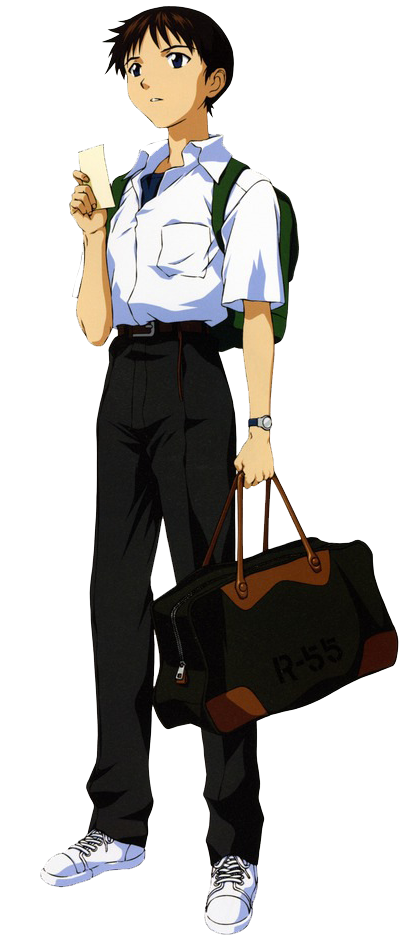
\includegraphics[width=1.25cm]{Shinji_Ikari.png}};};] (SI) at (0,0) {};

\node[label={\fontlabel{Asuka Langley Sohryu}},shape=circle, inner sep=1cm, path picture={\node at (path picture bounding box.center){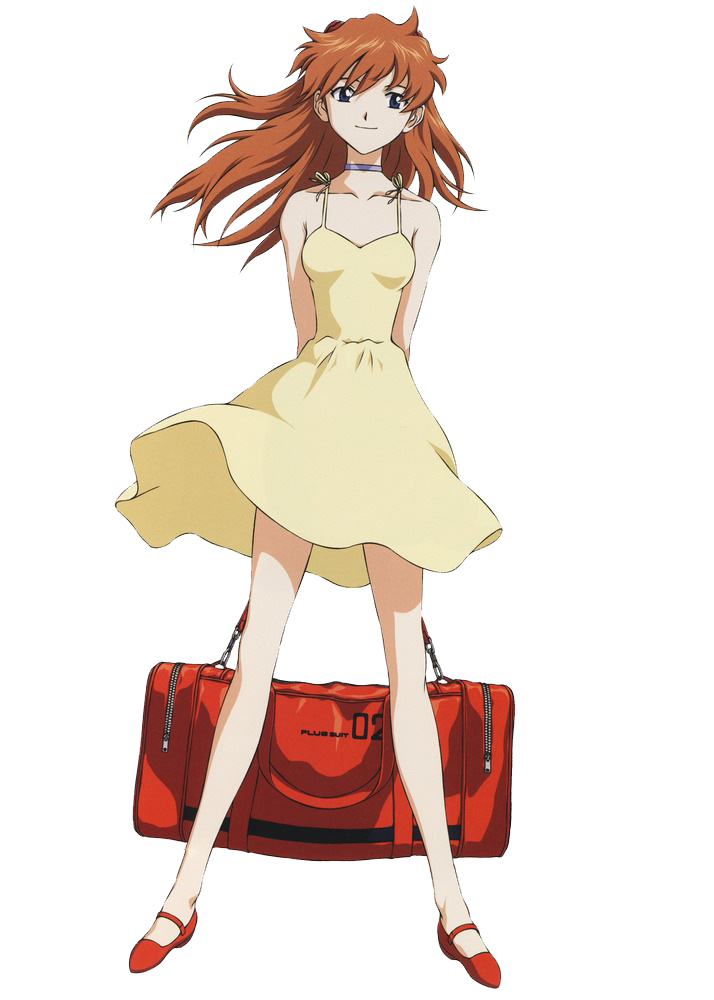
\includegraphics[width=2cm]{Asuka_Langley_Soryu.png}};};] (ALS) at (-3.5cm,7cm) {};

\node[label={\fontlabel{Rei Ayanami}},shape=circle, inner sep=1cm, path picture={\node at (path picture bounding box.center){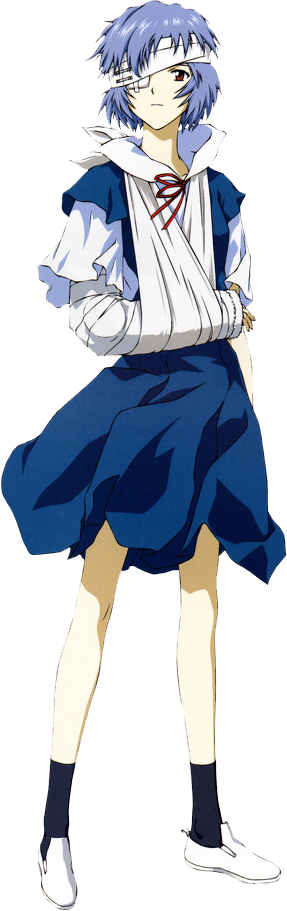
\includegraphics[width=0.9cm]{Rei_Ayanami.png}};};] (RA) at (3.5cm,7cm) {};
\node[label={\fontlabel{T\={o}ji Suzuhara}},shape=circle, inner sep=1cm, path picture={\node at (path picture bounding box.center){
\includegraphics[width=0.6cm]{Toji_Suzuhara.png}};};] (TS) at (0cm,14cm) {};
\end{scope}
\begin{scope}[every node/.style={draw=yellow,very thick}] %Evangelion units

\node[label={\fontlabel{Unit 00}},shape=circle, inner sep=1cm, path picture={\node at (path picture bounding box.center){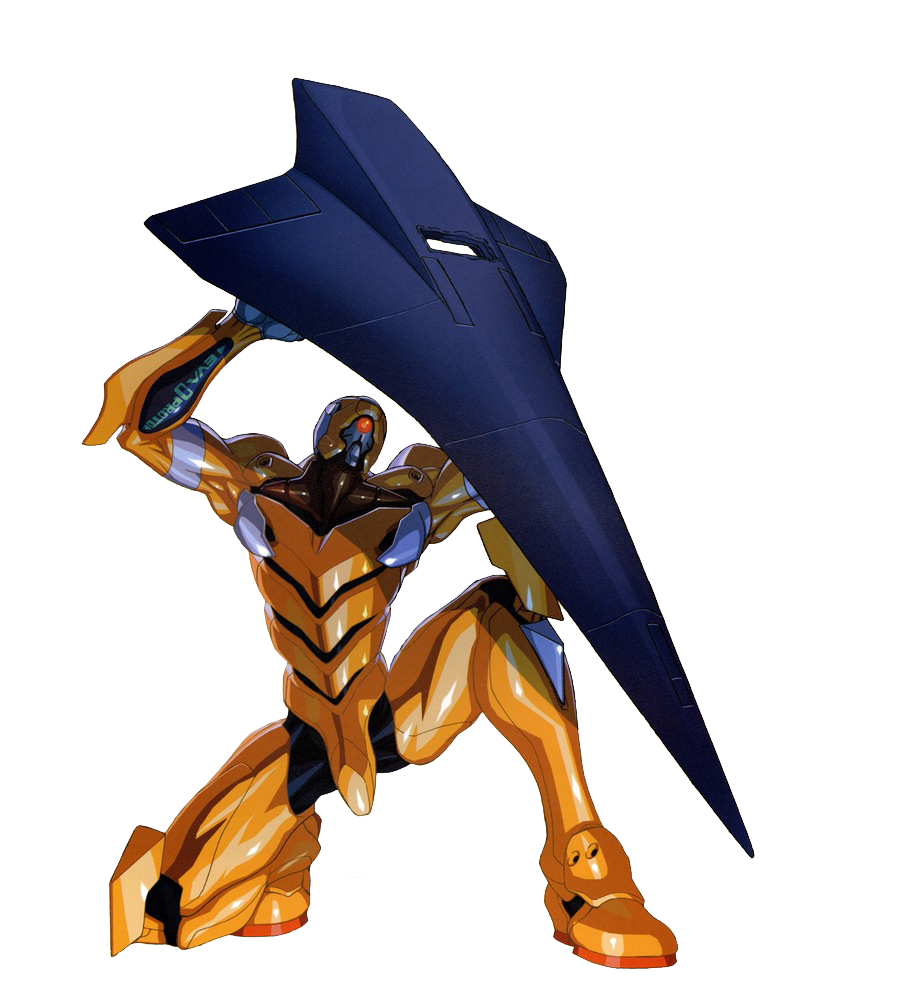
\includegraphics[width=2.5cm]{Unit_00.png}};};] (U0) at (-15cm,-10cm) {};

\node[label={\fontlabel{Unit 01}},shape=circle, inner sep=1cm, path picture={\node at (path picture bounding box.center){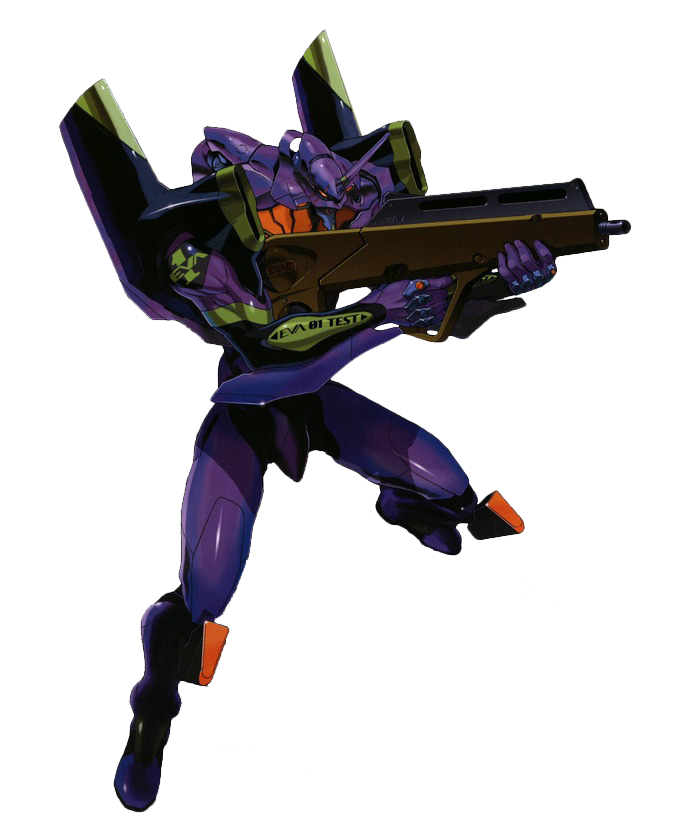
\includegraphics[width=2.5cm]{Unit_01.png}};};] (U1) at (-10cm,-10cm) {};

\node[label={\fontlabel{Unit 02}},shape=circle, inner sep=1cm, path picture={\node at (path picture bounding box.center){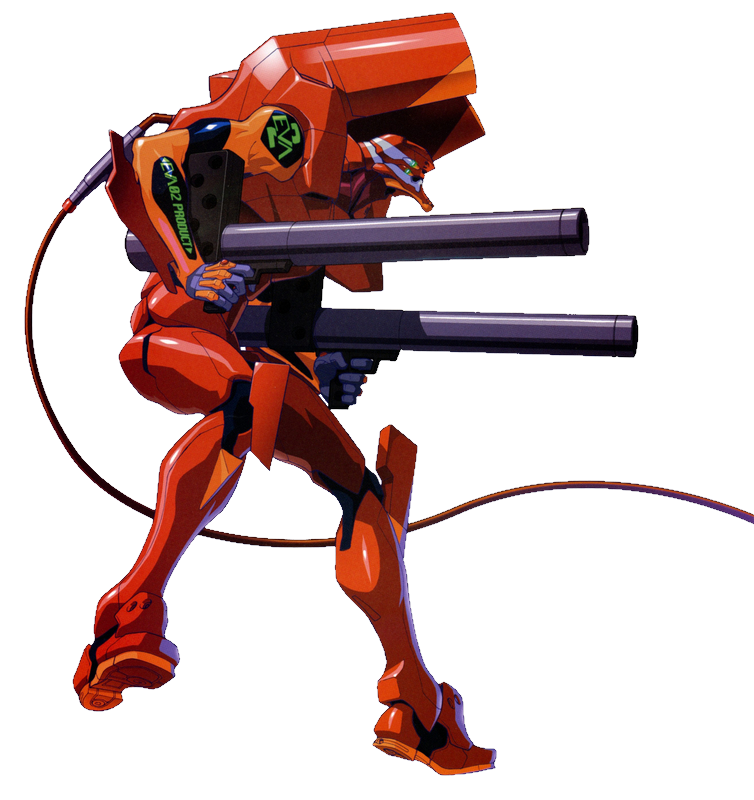
\includegraphics[width=2.5cm]{Unit_02.png}};};] (U2) at (10cm,-10cm) {};

\node[label={\fontlabel{Unit 03}},shape=circle, inner sep=1cm, path picture={\node at (path picture bounding box.center){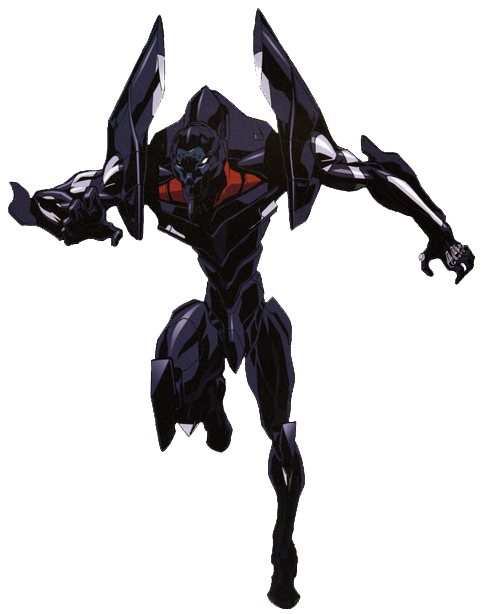
\includegraphics[width=2.5cm]{Unit_03.png}};};] (U3) at (15cm,-10cm) {};

\end{scope}
\begin{scope}[every node/.style={draw=red,very thick}] %NERV employees
\node[label={\fontlabel{Misato Katsuragi}},shape=circle, inner sep=1cm, path picture={\node at (path picture bounding box.center){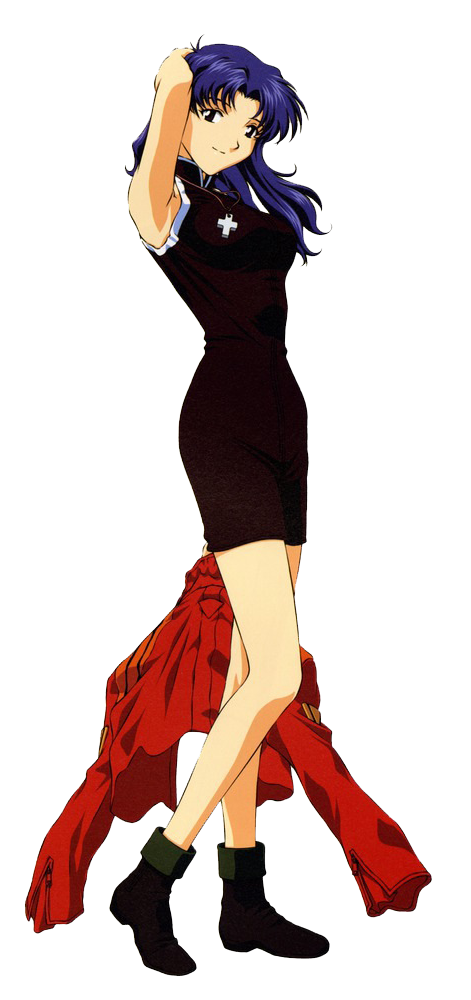
\includegraphics[width=1.5cm]{Misato_Katsuragi.png}};};] (MK) at (-5cm,0) {};

\node[label={\fontlabel{Gendo Ikari}},shape=circle, inner sep=1cm, path picture={\node at (path picture bounding box.center){
\includegraphics[width=1.2cm]{Gendo_Ikari.png}};};] (GI) at (5cm,2.5cm) {};

\node[label={\fontlabel{Ryoji Kaji}},shape=circle, inner sep=1cm, path picture={\node at (path picture bounding box.center){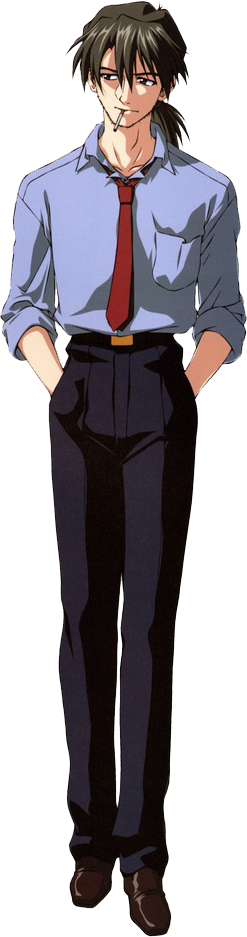
\includegraphics[width=0.75cm]{Ryoji_Kaji.png}};};] (RK) at (-5cm,-5cm) {};

\node[label={\fontlabel{Yui Ikari}},shape=circle, inner sep=1cm, path picture={\node at (path picture bounding box.center){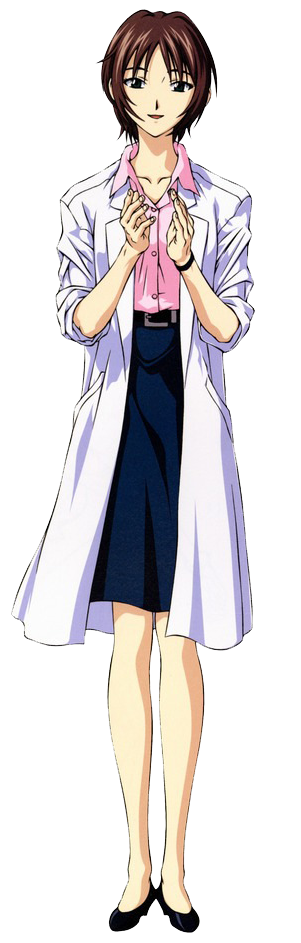
\includegraphics[width=0.9cm]{Yui_Ikari.png}};};] (YI) at (5cm,-2.5cm) {};

\node[label={\fontlabel{Akagi Ritsuko}},shape=circle, inner sep=1cm, path picture={\node at (path picture bounding box.center){
\includegraphics[width=1.4cm]{Ritsuko_Akagi.png}};};] (RAS) at (-10cm,-5cm) {};

\node[label={\fontlabel{Naoko Akagi}},shape=circle, inner sep=1cm, path picture={\node at (path picture bounding box.center){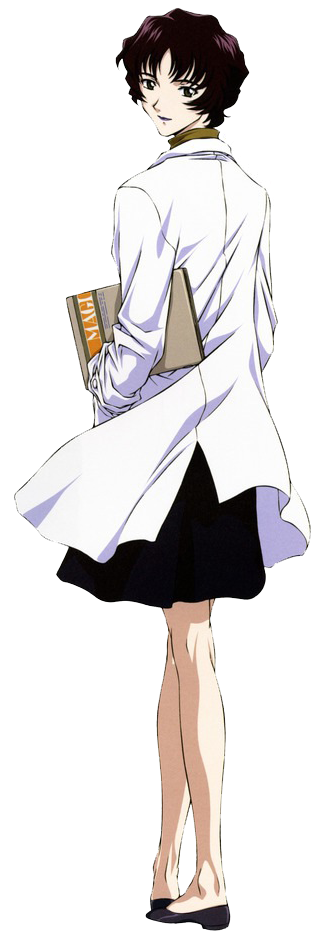
\includegraphics[width=1cm]{Naoko_Akagi.png}};};] (NA) at (7.5cm,7.5cm) {};

\node[label={\fontlabel{Fuyutsuki K\={o}z\={o}}},shape=circle, inner sep=1cm, path picture={\node at (path picture bounding box.center){
\includegraphics[width=1.1cm]{Kozo_Fuyutsuki.png}};};] (KF) at (10cm,-2.5cm) {};

\node[label={\fontlabel{Maya Ibuki}},shape=circle, inner sep=1cm, path picture={\node at (path picture bounding box.center){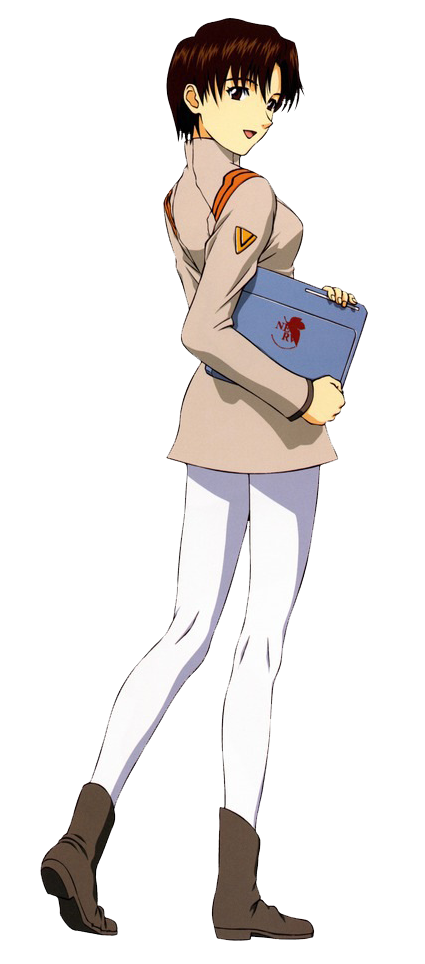
\includegraphics[width=1.2cm]{Maya_Ibuki.png}};};] (MI) at (13cm,-5cm) {};

\node[label={\fontlabel{Makoto Hyuga}},shape=circle, inner sep=1cm, path picture={\node at (path picture bounding box.center){
\includegraphics[width=0.9cm]{Makoto_Hyuga.png}};};] (MH) at (17cm,-3cm) {};

\node[label={\fontlabel{Shigeru Aoba}},shape=circle, inner sep=1cm, path picture={\node at (path picture bounding box.center){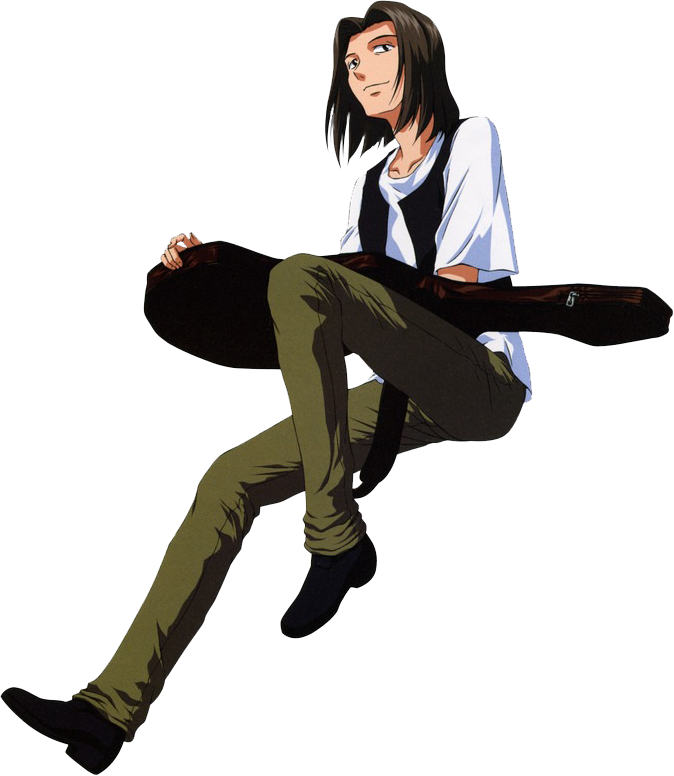
\includegraphics[width=2cm]{Shigeru_Aoba.png}};};] (SA) at (17cm,-7cm) {};

\end{scope}

\begin{scope}[every node/.style={draw=gray,very thick}] %Angels
\node[label={\fontlabel{Kaworu Nagisa (aka. Tabris)}},shape=circle, inner sep=1cm, path picture={\node at (path picture bounding box.center){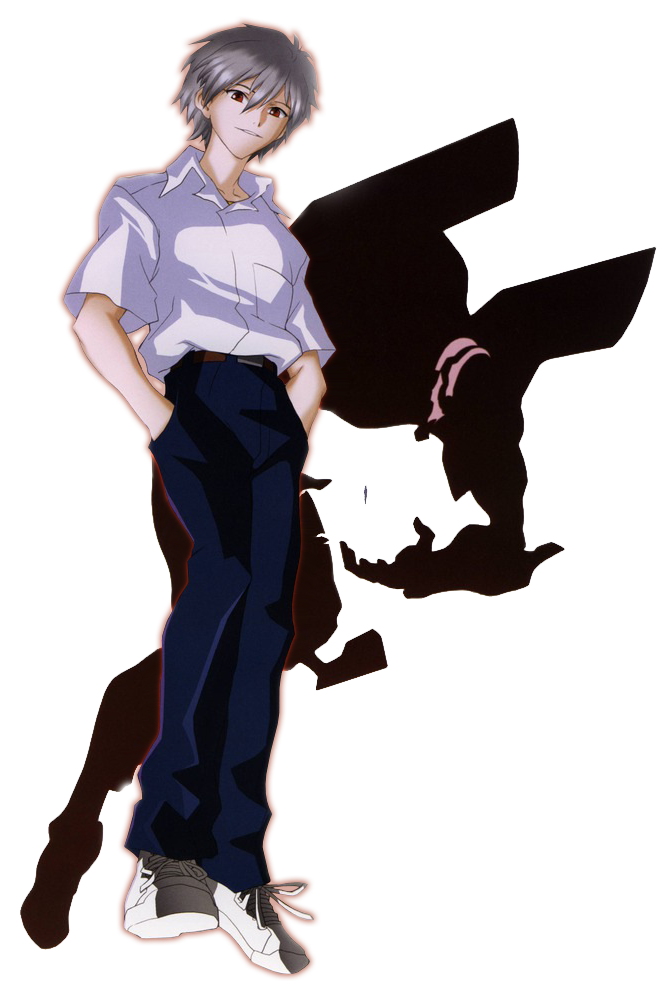
\includegraphics[width=1.9cm]{Kaworu_Nagisa.png}};};] (KN) at (0cm,-14cm) {};

\node[label={\fontlabel{Adam}},shape=circle, inner sep=1cm, path picture={\node at (path picture bounding box.center){
\includegraphics[width=2cm]{Adam.png}};};] (A1) at (0cm,-28cm) {};

\node[label={\fontlabel{Sachiel}}, shape=circle,inner sep=1cm,path picture={\node at (path picture bounding box.center){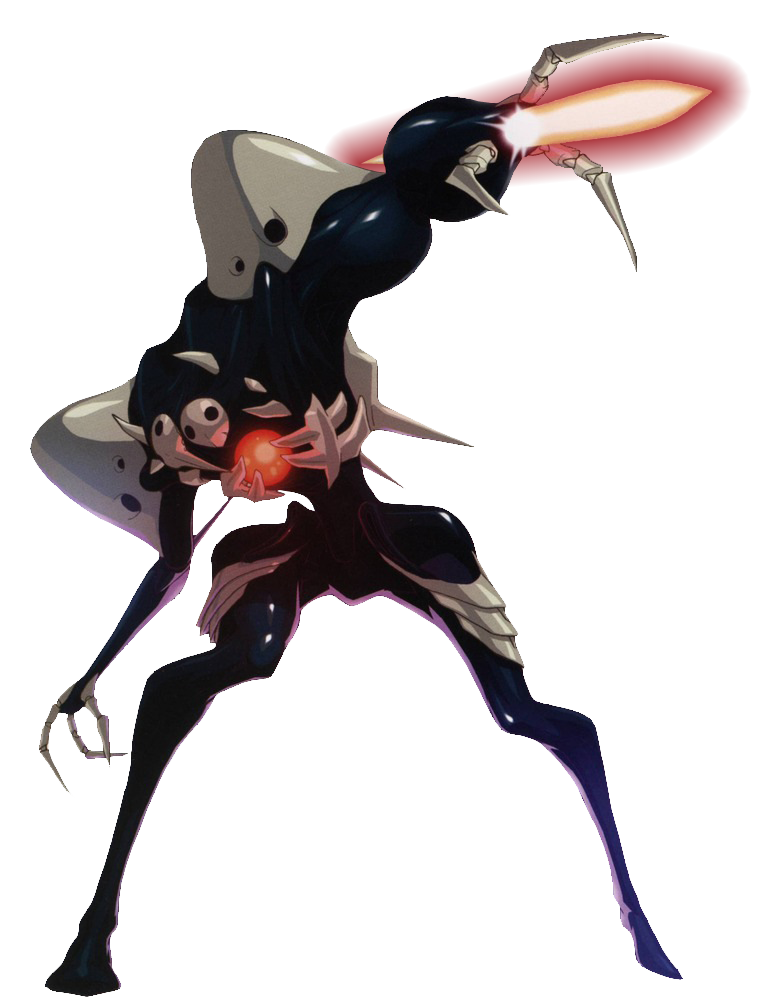
\includegraphics[width=2cm]{Sachiel.png}};};] (A3) at (-18.5cm,-25cm) { };

\node[label={\fontlabel{Shamshel}},shape=circle, inner sep=1cm, path picture={\node at (path picture bounding box.center){
\includegraphics[width=2cm]{Shamshel.png}};};] (A4) at (-18.5cm,-30cm) {};

\node[label={\fontlabel{Ramiel}},shape=circle, inner sep=1cm, path picture={\node at (path picture bounding box.center){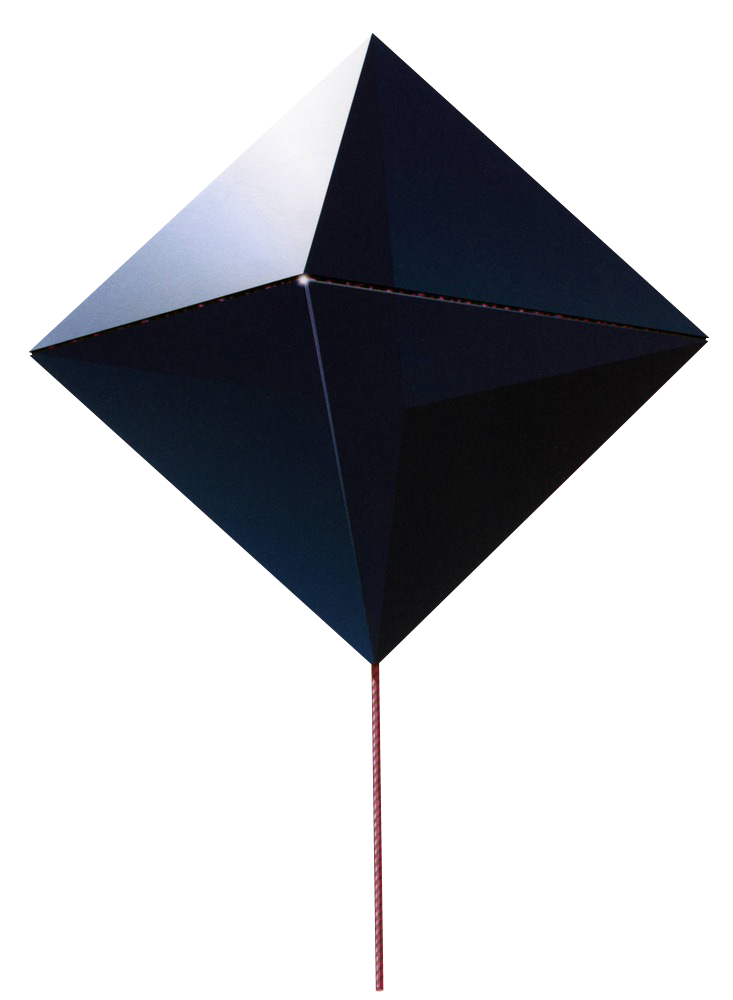
\includegraphics[width=2cm]{Ramiel.png}};};] (A5) at (-18.5cm,-35cm) {};

\node[label={\fontlabel{Gaghiel}},shape=circle, inner sep=1cm, path picture={\node at (path picture bounding box.center){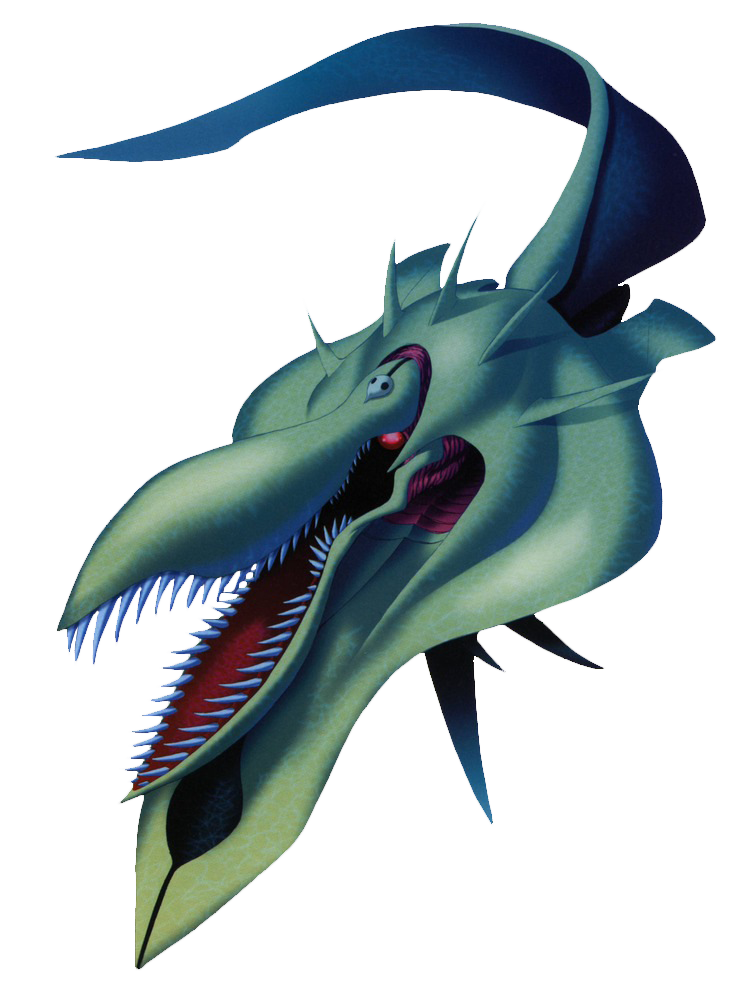
\includegraphics[width=2cm]{Gaghiel.png}};};] (A6) at (-14cm,-35cm) {};

\node[label={\fontlabel{Israfel}},shape=circle, inner sep=1cm, path picture={\node at (path picture bounding box.center){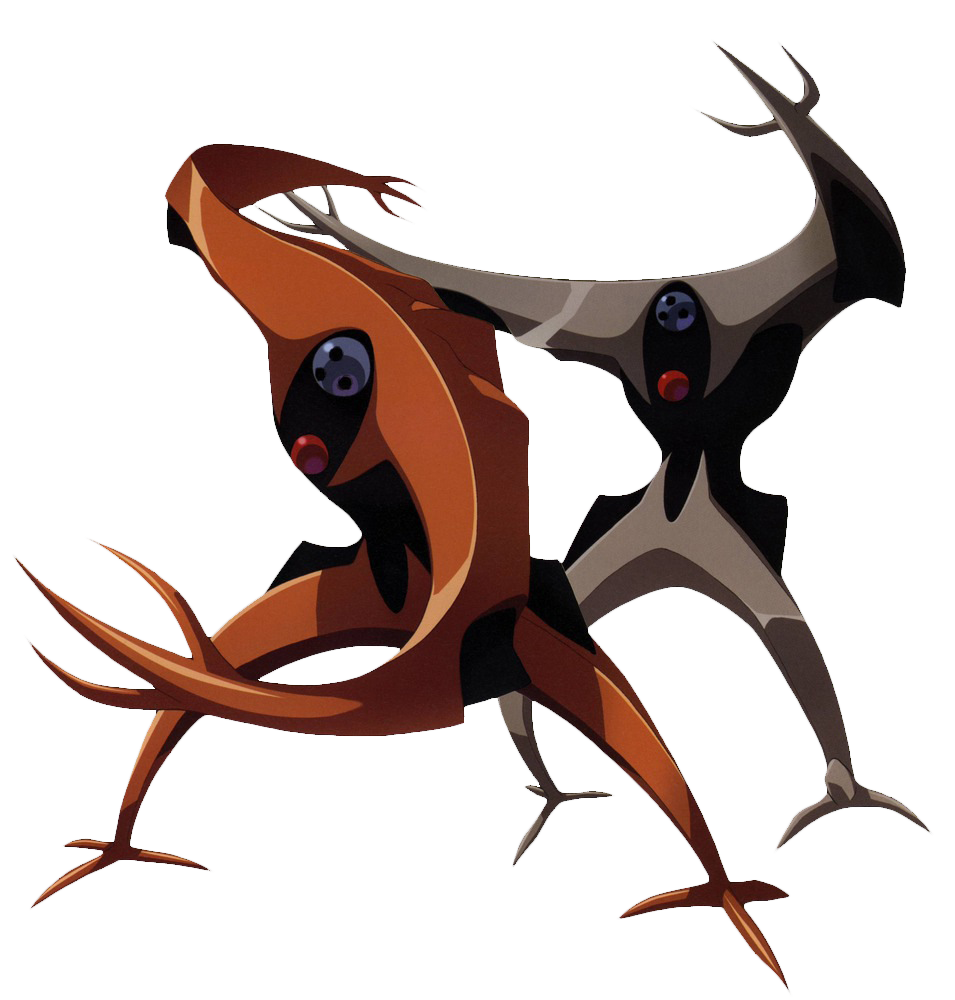
\includegraphics[width=2cm]{Israfel.png}};};] (A7) at (-9.5cm,-35cm) {};

\node[label={\fontlabel{Sandalphon}},shape=circle, inner sep=1cm, path picture={\node at (path picture bounding box.center){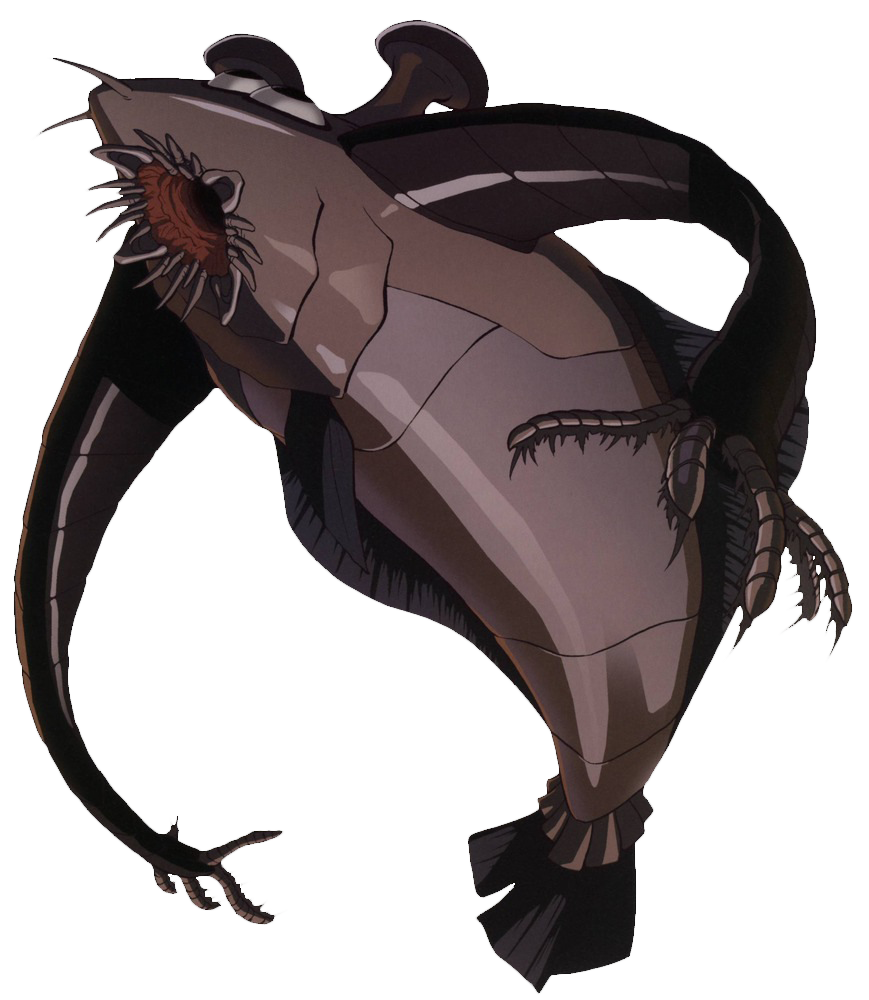
\includegraphics[width=2cm]{Sandalphon.png}};};] (A8) at (-5cm,-35cm) {};

\node[label={\fontlabel{Matarael}},shape=circle, inner sep=1cm, path picture={\node at (path picture bounding box.center){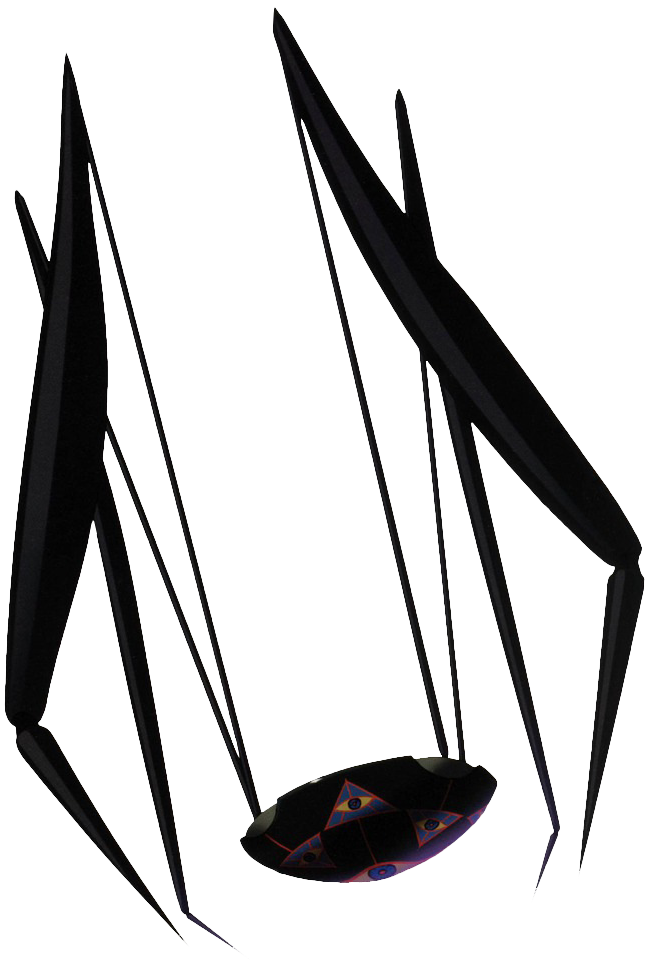
\includegraphics[width=2cm]{Matarael.png}};};] (A9) at (-1.5cm,-35cm) {};

\node[label={\fontlabel{Sahaquiel}},shape=circle, inner sep=1cm, path picture={\node at (path picture bounding box.center){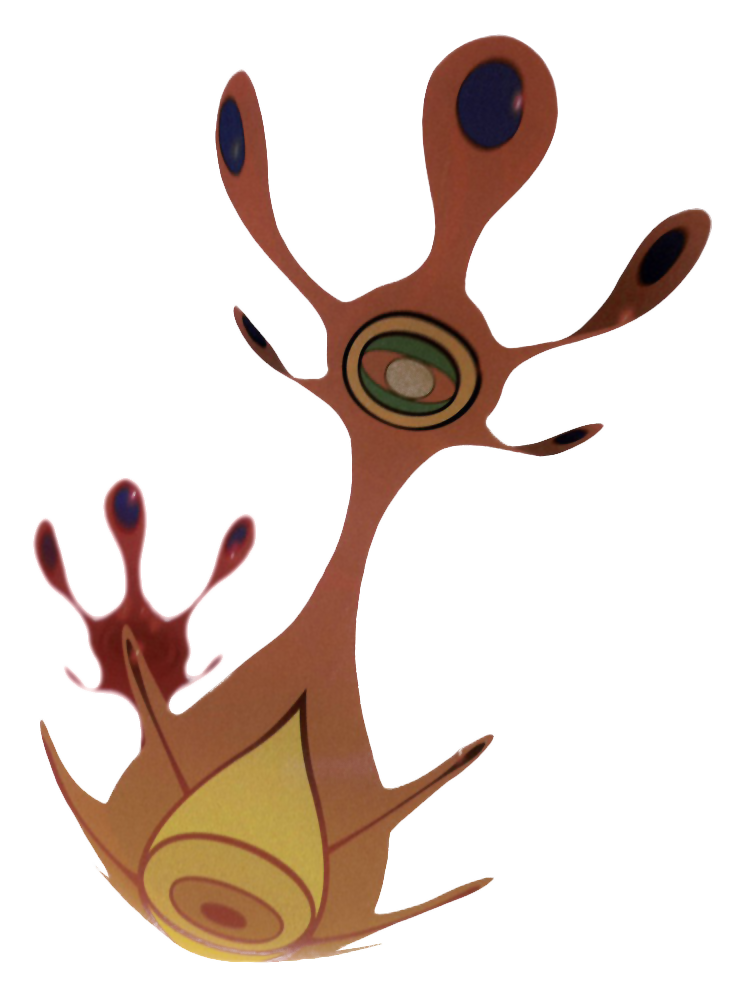
\includegraphics[width=2cm]{Sahaquiel.png}};};] (A10) at (1.5cm,-35cm) {};

\node[label={\fontlabel{Ireul}},shape=circle, inner sep=1cm, path picture={\node at (path picture bounding box.center){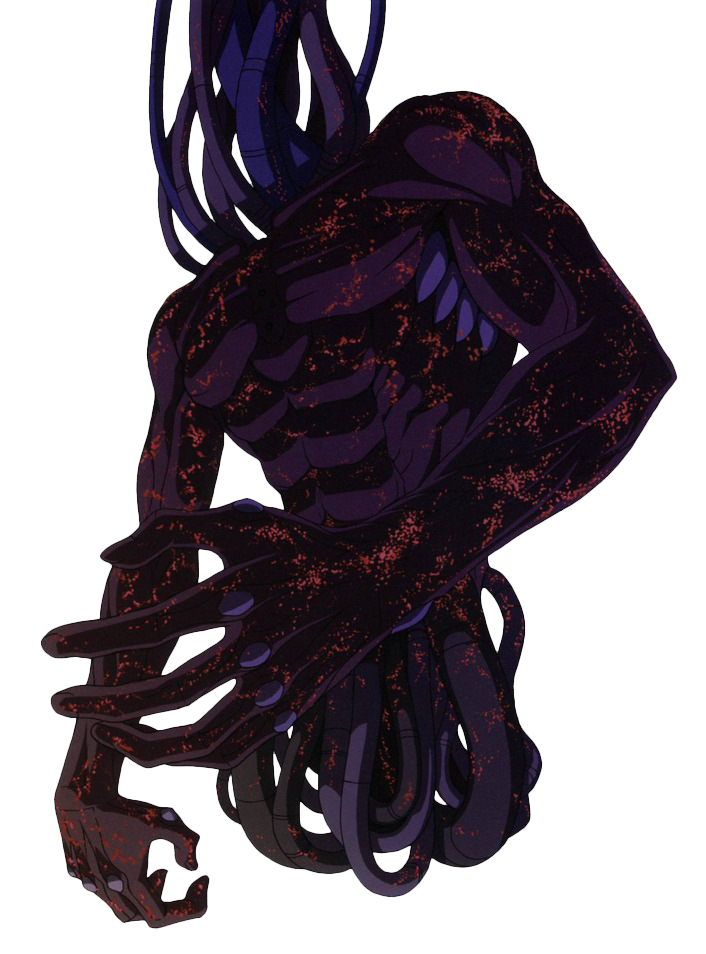
\includegraphics[width=2cm]{Ireul.png}};};] (A11) at (5cm,-35cm) {};

\node[label={\fontlabel{Leliel}},shape=circle, inner sep=1cm, path picture={\node at (path picture bounding box.center){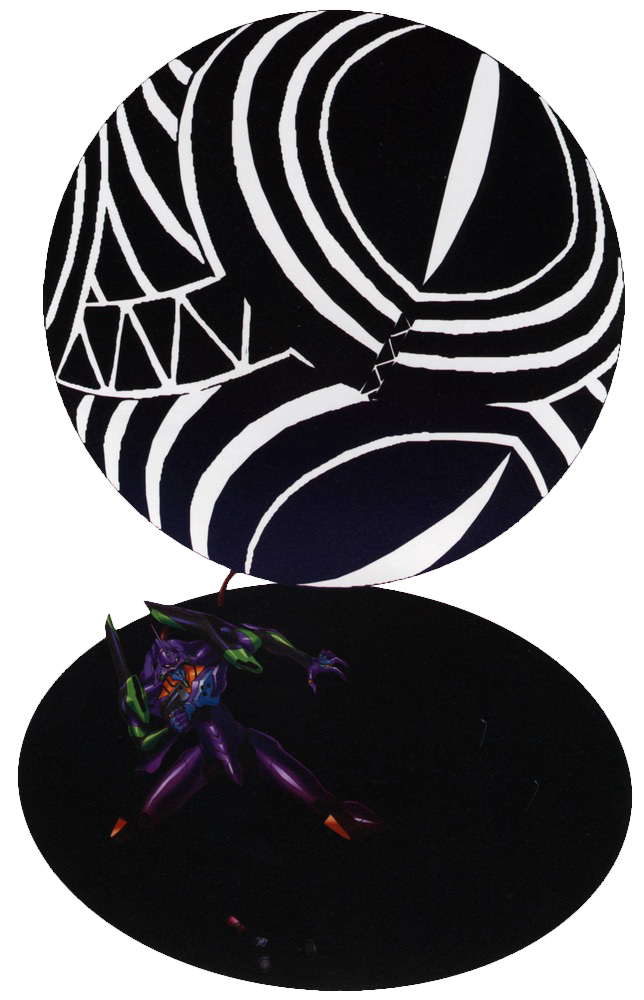
\includegraphics[width=2cm]{Leliel.png}};};] (A12) at (9.5cm,-35cm) {};

\node[label={\fontlabel{Bardiel}},shape=circle, inner sep=1cm, path picture={\node at (path picture bounding box.center){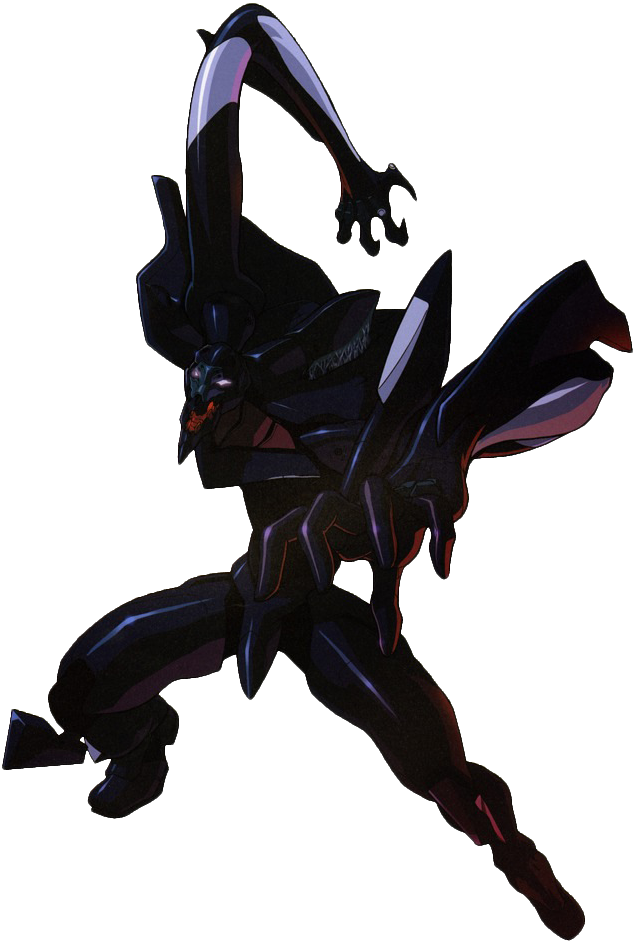
\includegraphics[width=2cm]{Bardiel.png}};};] (A13) at (14cm,-35cm) {};

\node[label={\fontlabel{Zeruel}},shape=circle, inner sep=1cm, path picture={\node at (path picture bounding box.center){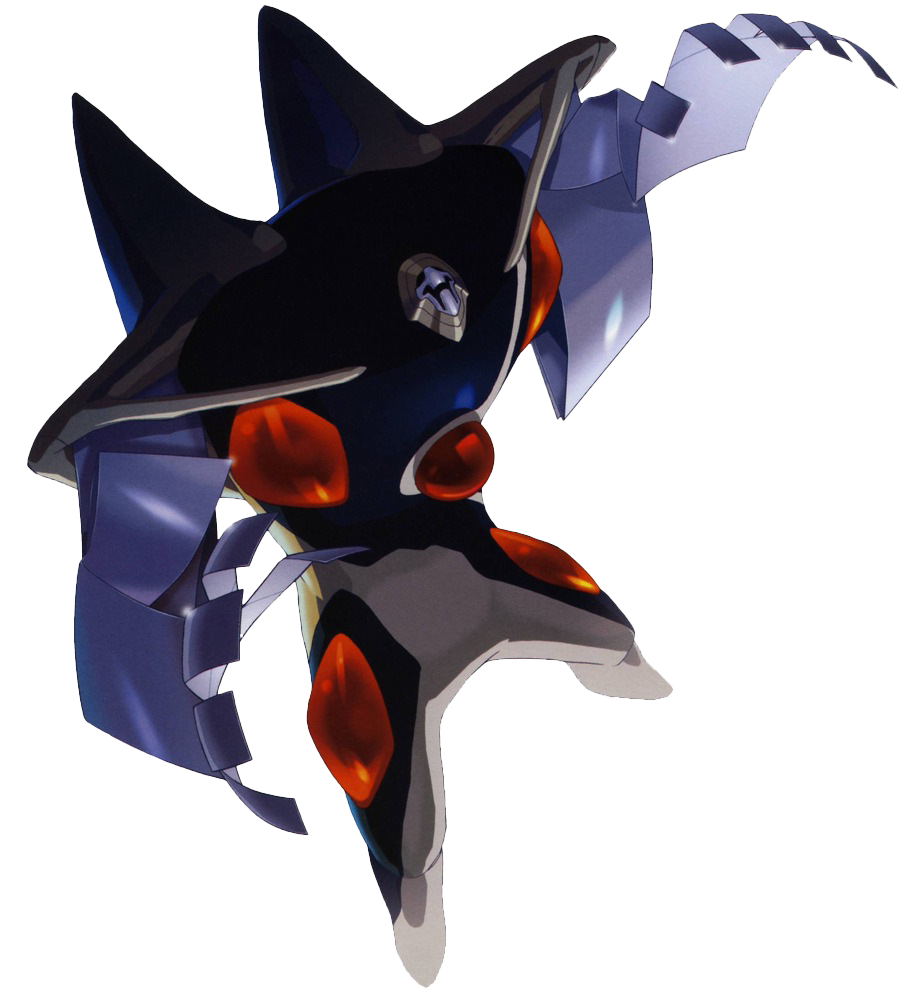
\includegraphics[width=2cm]{Zeruel.png}};};] (A14) at (18.5cm,-35cm) {};

\node[label={\fontlabel{Arael}},shape=circle, inner sep=1cm, path picture={\node at (path picture bounding box.center){
\includegraphics[width=2cm]{Arael.png}};};] (A15) at (18.5cm,-30cm) {};

\node[fill=gray,label={\fontlabel{Armisael}},shape=circle, inner sep=1cm, path picture={\node at (path picture bounding box.center){
\includegraphics[width=3cm]{Armisael.png}};};] (A16) at (18.5cm,-25cm) {};

\end{scope}

\begin{scope}[every node/.style={draw=black,very thick}] %miscellaneous
\node[label={\fontlabel{Pen\textsuperscript{2}}},shape=circle, inner sep=1cm, path picture={\node at (path picture bounding box.center){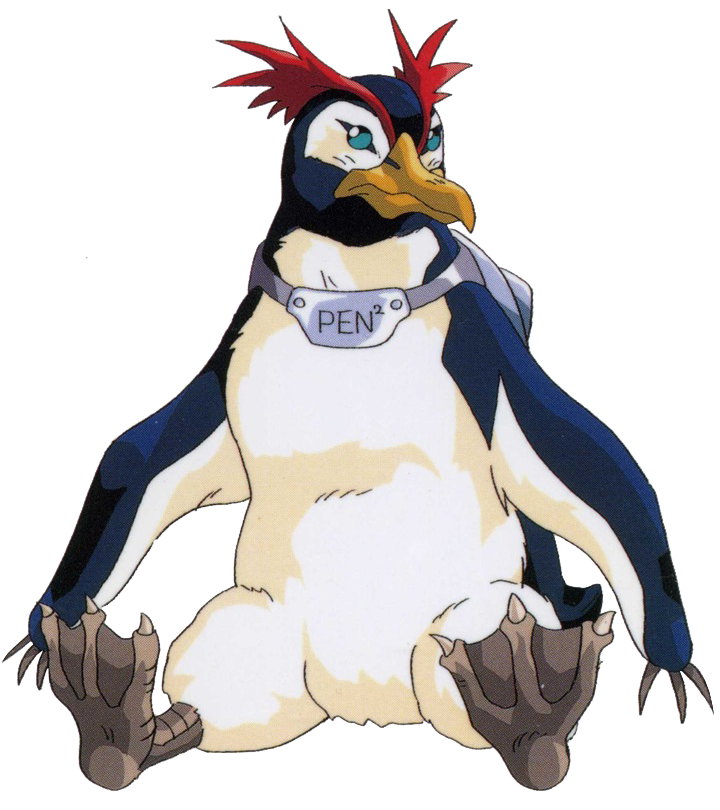
\includegraphics[width=2cm]{Pen_Pen.png}};};] (PP) at (-15cm,0cm) {};
\node[label={\fontlabel{Keel Lorenz}},shape=circle, inner sep=1cm, path picture={\node at (path picture bounding box.center){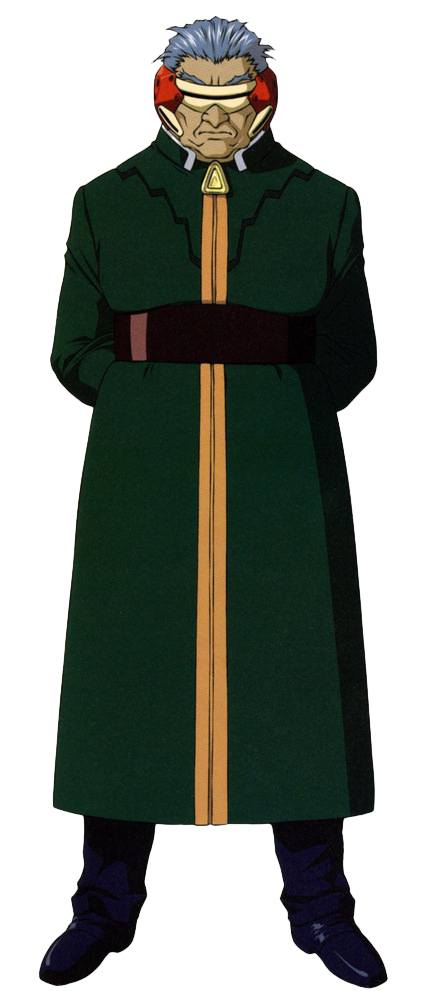
\includegraphics[width=1.25cm]{Keel_Lorenz.png}};};] (KL) at (14cm,1.25cm) {};
\node[label={\fontlabel{Hikari Horaki}},shape=circle, inner sep=1cm, path picture={\node at (path picture bounding box.center){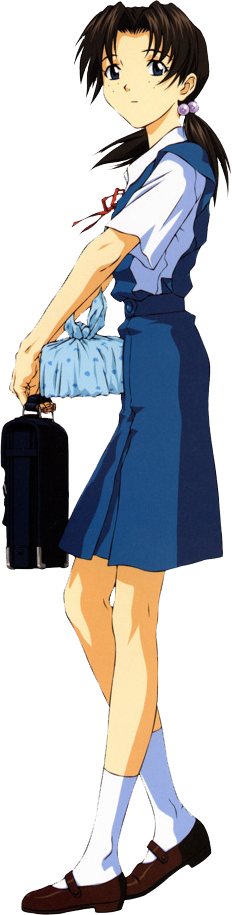
\includegraphics[width=0.7cm]{Hikari_Horaki.png}};};] (HH) at (-14cm,10cm) {};

\node[label={\fontlabel{Kensuke Aida}},shape=circle, inner sep=1cm, path picture={\node at (path picture bounding box.center){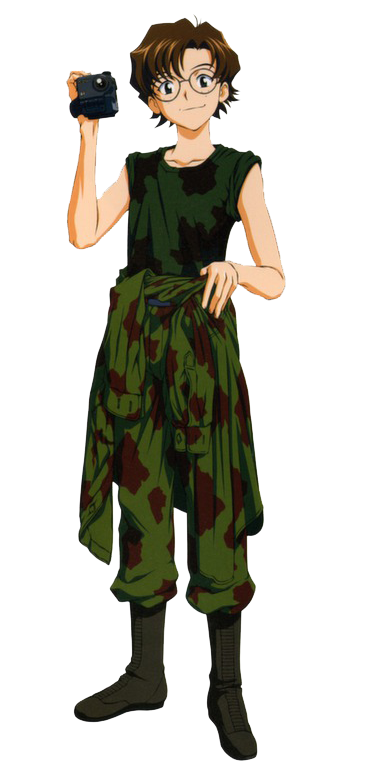
\includegraphics[width=1.25cm]{Kensuke_Aida.png}};};] (KA) at (14cm,10cm) {};

\end{scope}

\begin{scope}[every edge/.style={draw=red,very thick}] %romantic relationships
\path[<->] (SI) edge node {} (KN);
\path[<->] (SI) edge node {} (RA);
\path[<->] (SI) edge node {} (MK);
\path[<->] (SI) edge node {} (ALS);
\path[->] (ALS) edge[bend right=60] node {} (RK);
\path[<->] (RAS) edge node {} (RK);
\path[<->] (MK) edge node {} (RK);
\path[->] (RAS) edge[bend right=9999] node {} (GI);
\path[->] (KF) edge node {} (YI);
\path[<->] (YI) edge node {} (GI);
\path[<-] (YI) edge node {} (KF);
\path[<->] (GI) edge node {} (RA);
\path[<-] (GI) edge node {} (NA);
\path[->] (KA) edge[bend right=15] node[midway, above, sloped] {in manga adaptation} (ALS);
\end{scope}

\begin{scope}[every edge/.style={draw=green,very thick}] %creators
\path[<-] (A3) edge[bend left=10] node {} (A1);

\path[<-] (A4) edge[bend left=15] node {} (A1);
\path[<-] (A5) edge[bend left=10] node {} (A1);
\path[<-] (A6) edge[bend left=5] node {} (A1);
\path[<-] (A7) edge node {} (A1);
\path[<-] (A8) edge node {} (A1);
\path[<-] (A9) edge node {} (A1);
\path[<-] (A10) edge node {} (A1);
\path[<-] (A11) edge node {} (A1);
\path[<-] (A12) edge node {} (A1);
\path[<-] (A13) edge[bend right=5] node {} (A1);
\path[<-] (A14) edge[bend right=10] node {} (A1);
\path[<-] (A15) edge[bend right=15] node {} (A1);
\path[<-] (A16) edge[bend right=10] node {} (A1);
\path[<-] (KN) edge node {} (A1);
\path[<-] (SI) edge node {} (GI);
\path[<-] (SI) edge node {} (YI);
\path[<-] (RA) edge[bend left=15] node {} (GI);
\end{scope}

\begin{scope}[every edge/.style={draw=blue,very thick}] %subordination
\path[<-] (SI) edge[bend left=15] node {} (MK);
\path[<-] (ALS) edge node {} (MK);
\path[<-] (RA) edge node {} (MK);
\path[<-] (MK) edge[bend left=15] node {} (GI);
\path[<-] (GI) edge[bend left=0] node {} (KL);
\path[->] (GI) edge node {} (KF);

\path[<-] (U0) edge[bend left=15] node {} (RA);
\path[<-] (U1) edge[bend right=25] node {} (SI);
\path[<-] (U2) edge[bend left=45] node {} (ALS);
\path[<-] (U2) edge node[midway, above, sloped] {Episode 08 only} (SI);
\path[<-] (U3) edge[bend right=45] node {} (TS);

\path[->] (GI) edge[bend left=0] node {} (MH);
\path[->] (GI) edge[bend right=35] node {} (MI);
\path[->] (GI) edge[bend left=10] node {} (SA);
\end{scope}



\begin{scope}[every edge/.style={draw=black,very thick}] %destruction
\path[->] (U1) edge node {} (A3);
\path[->] (U1) edge node {} (A4);
\path[->] (U1) edge node {} (A5);
\path[->] (U2) edge node {} (A6);
\path[->] (U2) edge node {} (A7);
\path[->] (U1) edge node {} (A7);
\path[->] (U2) edge node {} (A8);
\path[->] (U1) edge node {} (A9);
\path[->] (U2) edge node {} (A10);
\path[->] (RAS) edge node {} (A11);
\path[->] (U1) edge node {} (A12);
\path[->] (A13) edge node {} (U3);
\path[->] (U1) edge[bend left=30] node {} (U3);
\path[->] (U3) edge node {} (A13);
\path[->] (U1) edge node {} (A14);
\path[->] (U0) edge node {} (A15);
\path[<->] (U0) edge node {} (A16);
\path[->] (U1) edge node {} (KN);
\end{scope}

\begin{scope}[every edge/.style={draw=gray,very thick}] %miscellaneous
\path[->] (MK) edge node {} (PP);
\path[->] (HH) edge node {} (PP);

\path[<->] (TS) edge node {} (KA);
\path[<->] (TS) edge node {} (HH);

\path[<->] (MI) edge node {} (MH);
\path[<->] (MI) edge node {} (SA);
\path[<->] (MH) edge node {} (SA);

\end{scope}
\end{tikzpicture}
\end{document}
